\chapter{Experiment}\label{chap:experiment}

Three sets of experiments have been conducted. A migration tweet detection was executed at the beginning of the project, exploring the performance of the three classifier. A sentiment detection model is built using annotated data, performance metric are computed. Tweets which are classified as migration tweets are passed to sentiment detection model to detect its sentiment.

\section{Migration detection model}
This section describes the steps which were conducted while building migration detection model.
\subsection{Data-set collection}

For the migration detection model, twitter archives \footnote{\url{https://archive.org/}} was considered to collect the data.
The data-set was collected by filtering out, using following hash-tags
\#refugee, \#wall, \#Syria, \#syrianrefugee,
\#mexicanwall, \#trumpwall, \#immigrants. A total of 1275 tweets were collected from data archive(100GB). The year 2016 was chosen because the hash tags used to search tweets were trending during that period. The tweets filtered are stored in JSON format.



\subsection{Prepossessing} \label{sssec:preprocessing}

Data prepossessing is fundamental step to all data science and
Natural Language Processing Tasks. The prepossessing steps in
our project is common to both migration detection and sentiment detection models the models. After retrieving the JSON, the prepossessing script performs the following steps:
\begin{enumerate}
    \item Take only lines with "English" language Tweets.
    \item Sort the tweets, Check similarity between consecutive tweets , if similarity is greater than 80\%, remove the duplicate tweets.
    \item Search for the full\_text of the tweet (In cases of re-tweets or too big tweets, additional attributes are added to the tweet.
    \item Deleting all non-alphanumeric characters.
\end{enumerate}
The scripts are mainly implemented using the regular expression. The prepossessed tweets are manual annotated with label ``yes" and ``no". After this step the data is clean and is passed to feature engineering step. Distribution of obtained tweets are show in the figure \ref{fig:graphDistmigration}.

\begin{figure}
	\centering
	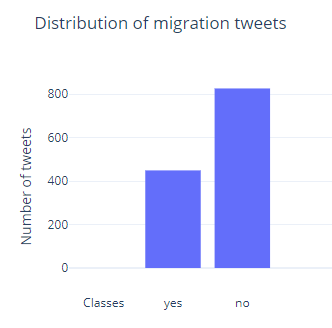
\includegraphics[width=10cm\linewidth,height=10cm]{thesis_template/images/distofmigration_tweetsundefined.png}
	\caption{Distribution of the migration tweets}
	\label{fig:graphDistmigration}
\end{figure}


\subsection{Feature engineering }
Feature Engineering starts from an initial set of measured data and
build derived values (features) which is intended to be informative. In this project, Count vectorizer is used to extract feature from the text of the tweet. Along with that Migration index(MI) and migration percentage(MP) is calculated, section \ref{featureengineering} discusses the process of computing MI and MP. Count vector is a sparse matrix, this feature is combined with MP and MI feature using feature union technique, section \ref{backgroundworkFeatureEngi} discusses the technique of feature union.  

\subsection{Classification and Metrics}
The classifier is treated as a binary classifier, with the labels ``yes" and ``no". The label ``yes" represents the tweets is a migration tweet and the label ``no" represnts the tweets is not related to migration. For classification results in any classification analysis, accuracy, precision, recall and F1 are computed. Since the F1 score is a harmonic means of precision and recall, it is sometimes enough to report this metric. In our experiments, we follow this convention and report all the above measurements and a macro- averaged F1 score.

Three classifier are used in this project, naive Bayes, Logistic regression, decision trees. Performance metric of all the three classifier is given in table \ref{tab:Migration_metric}


\begin{table}[]
\centering
\begin{tabular}{lllll}
\hline
\textbf{Classifier} & \textbf{Accuracy} & \textbf{Precision} & \textbf{Recall} & \textbf{F1-score} \\ \hline
Logistic regression & 0.937             & 0.956              & 0.844           & 0.896             \\ \hline
Naive Bayes         & 0.821             & 0.709              & 0.757           & 0.732             \\ \hline
Decision Trees     & 0.943             & 0.938              & 0.883           & 0.909             \\ \hline
\end{tabular}
\caption{Performance metric of all the classifier - Migration model}
\label{tab:Migration_metric}
\end{table}

\subsubsection{Naive Bayes}
The performance score and confusion matrix of migration detection from the naive Bayes model is show in the table \ref{tab:confusionmatrix_migrationtweets} and \ref{tab:performancemetricofmigration}

\begin{table}[]
\centering
\begin{tabular}{lllll}
\cline{1-3}
\multicolumn{1}{|l|}{}   & \multicolumn{1}{l|}{predicted\_YES} & \multicolumn{1}{l|}{predicted\_NO}  &  &  \\ \cline{1-3}
\multicolumn{1}{|l|}{YES} & \multicolumn{1}{l|}{78}  & \multicolumn{1}{l|}{25} &  &  \\ \cline{1-3}
\multicolumn{1}{|l|}{NO}   & \multicolumn{1}{l|}{32}  & \multicolumn{1}{l|}{184}  &  &  \\ \cline{1-3}
                            &                           &                           &  & 
\end{tabular}
\caption{Naive Bayes: Confusion matrix for migration model}
\label{tab:confusionmatrix_migrationtweets}
\end{table}





\subsubsection{Logistic regression}
The performance score and confusion matrix of migration detection model using the logistic regression algorithm is show in the table \ref{tab:confusionmatrix_migrationtweets} and \ref{tab:performancemetricofmigration}

\begin{table}[]
\centering
\begin{tabular}{lllll}
\cline{1-3}
\multicolumn{1}{|l|}{}   & \multicolumn{1}{l|}{predicted\_YES} & \multicolumn{1}{l|}{predicted\_NO}  &  &  \\ \cline{1-3}
\multicolumn{1}{|l|}{YES} & \multicolumn{1}{l|}{87}  & \multicolumn{1}{l|}{16} &  &  \\ \cline{1-3}
\multicolumn{1}{|l|}{NO}   & \multicolumn{1}{l|}{4}  & \multicolumn{1}{l|}{212}  &  &  \\ \cline{1-3}
                            &                           &                           &  & 
\end{tabular}
\caption{Logistic regression: Confusion matrix for migration model}
\label{tab:confusionmatrix_migrationtweets}
\end{table}





\subsubsection{Decision trees}
The performance score and confusion matrix of the migration detection model using decision trees algorithm can be found in the table.
 \ref{tab:confusionmatrix_migrationtweets} and \ref{tab:performancemetricofmigration}

\begin{table}[]
\centering
\begin{tabular}{lllll}
\cline{1-3}
\multicolumn{1}{|l|}{}   & \multicolumn{1}{l|}{predicted\_YES} & \multicolumn{1}{l|}{predicted\_NO}  &  &  \\ \cline{1-3}
\multicolumn{1}{|l|}{YES} & \multicolumn{1}{l|}{87}  & \multicolumn{1}{l|}{16} &  &  \\ \cline{1-3}
\multicolumn{1}{|l|}{NO}   & \multicolumn{1}{l|}{4}  & \multicolumn{1}{l|}{212}  &  &  \\ \cline{1-3}
                            &                           &                           &  & 
\end{tabular}
\caption{Decision trees: Confusion matrix for migration model}
\label{tab:confusionmatrix_migrationtweets}
\end{table}






\section{Sentiment detection model}
\subsection{Data-set collection}
For the sentiment detection model, Annotated data-set from the Stanford Twitter Corpus \footnote{\url{http://help.sentiment140.com/for-students/}} was used. Distribution of the tweets is shown in the figure \ref{fig:graphDistsentiment}

\subsection{Prepossessing}
Prepossessing steps are same as mentioned in section 

fig \ref{fig:graphDistsentiment}
\begin{figure}
	\centering
	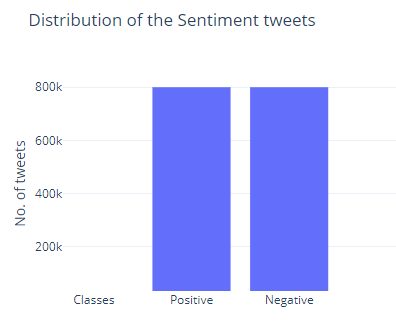
\includegraphics[width=12cm\linewidth,height=10cm]{thesis_template/images/distofsentiment_tweetsundefined.png}
	\caption{Distribution of the sentiment tweets}
	\label{fig:graphDistsentiment}
\end{figure}


\subsection{Feature engineering }
\subsection{Classification and Metrics}

\subsubsection{Logistic regression}

\begin{table}[]
\centering
\begin{tabular}{lllll}
\cline{1-3}
\multicolumn{1}{|l|}{}   & \multicolumn{1}{l|}{predicted\_YES} & \multicolumn{1}{l|}{predicted\_NO}  &  &  \\ \cline{1-3}
\multicolumn{1}{|l|}{YES} & \multicolumn{1}{l|}{6624}  & \multicolumn{1}{l|}{1294} &  &  \\ \cline{1-3}
\multicolumn{1}{|l|}{NO}   & \multicolumn{1}{l|}{1443}  & \multicolumn{1}{l|}{6599}  &  &  \\ \cline{1-3}
                            &                           &                           &  & 
\end{tabular}
\caption{Logistic regression: Confusion matrix for sentiment model}
\label{tab:confusionmatrix_migrationtweets}
\end{table}



\subsubsection{Naive Bayes}



\begin{table}[]
\centering
\begin{tabular}{lllll}
\cline{1-3}
\multicolumn{1}{|l|}{}   & \multicolumn{1}{l|}{predicted\_YES} & \multicolumn{1}{l|}{predicted\_NO}  &  &  \\ \cline{1-3}
\multicolumn{1}{|l|}{YES} & \multicolumn{1}{l|}{78}  & \multicolumn{1}{l|}{25} &  &  \\ \cline{1-3}
\multicolumn{1}{|l|}{NO}   & \multicolumn{1}{l|}{32}  & \multicolumn{1}{l|}{184}  &  &  \\ \cline{1-3}
                            &                           &                           &  & 
\end{tabular}
\caption{Naive Bayes: Confusion matrix for sentiment model}
\label{tab:confusionmatrix_migrationtweets}
\end{table}



\subsubsection{Decision trees}



\begin{table}[]
\centering
\begin{tabular}{lllll}
\cline{1-3}
\multicolumn{1}{|l|}{}   & \multicolumn{1}{l|}{predicted\_YES} & \multicolumn{1}{l|}{predicted\_NO}  &  &  \\ \cline{1-3}
\multicolumn{1}{|l|}{YES} & \multicolumn{1}{l|}{78}  & \multicolumn{1}{l|}{25} &  &  \\ \cline{1-3}
\multicolumn{1}{|l|}{NO}   & \multicolumn{1}{l|}{32}  & \multicolumn{1}{l|}{184}  &  &  \\ \cline{1-3}
                            &                           &                           &  & 
\end{tabular}
\caption{Decision trees: Confusion matrix for sentiment model}
\label{tab:confusionmatrix_migrationtweets}
\end{table}






\section{Sentiment analysis of migration classified tweets}

Tweets classified as migration tweets from the migration detection model are passed to the sentiment detection model. The migration tweets are also annotated with their respective sentiment labels in tweet annotation step. This step to annotate the sentiment of migration tweets is considered as the ground truth, and the performance of the sentiment detection model which is built using logistic regression algorithm is calculated using the ground truth and the predicted value. 
The number of tweets which are classified as the migration tweets is 449 tweets, and the distribution of the annotated sentiment labels is shown in the figure \ref{fig:sent_migration_distribution}. The performance metric of detecting the sentiment of these tweets are shown in table \ref{tab:sentiment_of_Migration_metric}

 

\begin{figure}
	\centering
	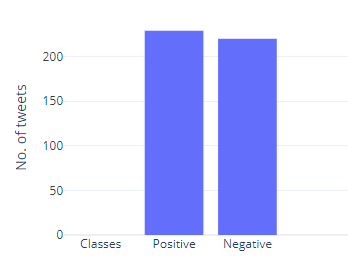
\includegraphics[width=12cm\linewidth,height=10cm]{thesis_template/images/sentiment_of_migration_tweets.png}
	\caption{ The distribution of "sentiment labels" for the classified migration tweets.}
	\label{fig:sent_migration_distribution}
\end{figure}

\begin{table}[]
\centering
\begin{tabular}{lllll}
\hline
\textbf{Classifier} & \textbf{Accuracy} & \textbf{Precision} & \textbf{Recall} & \textbf{F1-score} \\ \hline
Logistic regression & 57.02             & 0.58              & 0.57          & 0.55              \\ \hline

\end{tabular}
\caption{Performance metric of detecting the sentiment of migration tweets}
\label{tab:sentiment_of_Migration_metric}
\end{table}